%!TEX root = ../these.tex

\section{%
Формализация общей задачи маршрутизации режущего инструмента
}
\label{sec:cut.stmt}

Для формального определения маршрута резки введем следующие обозначения
\cite{bi:book2020,bib:petunin-2019}.
Пусть
$A_1, A_2, \,\dots, A_n$
--- двумерные геометрические объекты
(точечные замкнутые множества),
представляющие собой односвязные или
многосвязные области евклидовой плоскости
$\mathbb R \times \mathbb R$,
ограниченные одной или несколькими замкнутыми кривыми
(граничными контурами)
$C_1, C_2, \,\dots, C_N$
$(A_i, C_J \subset \mathbb R \times \mathbb R;
i \in \overline{1,n};
j \in \overline{1, N};
N \geqslant n)$.
Объекты
$A_1, A_2, \,\dots, A_n$
являются геометрическими моделями плоских заготовок / деталей.

Пусть также определена область размещения объектов
$\mathcal B \subset \mathbb R \times \mathbb R$,
которая является геометрической моделью листового материала,
из которого вырезаются детали.
Как правило, это прямоугольник,
но иногда на практике могут встречаться
более сложные случаи.

Будем полагать, что раскройная карта зафиксирована,
при этом выполнены условия взаимного непересечения объектов.
Полагаем также, что выполнены другие дополнительные условия,
обусловленные технологическими требованиями резки деталей
на конкретном технологическом оборудовании с ЧПУ,
в частности, условие соблюдения необходимой ширины реза.
Другими словами, фиксированный вариант размещения объектов
является допустимым вариантом раскроя листового материала
для заданного набора $n$ деталей.

Пример размещения в прямоугольной области 24 объектов
($n=24$),
описываемых 30 замкнутыми контурами
($N=30$)
с заданным минимальным расстоянием между объектами,
приведен на рис.~\ref{fig:cut.nesting}.

\begin{figure}
  \centering
  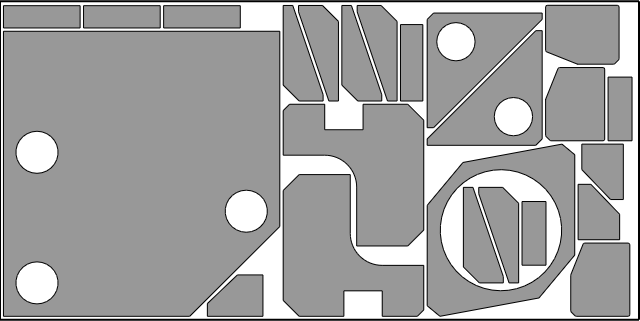
\includegraphics[width=0.9\textwidth]{nesting-24.png}
  \caption{
    Пример раскроя листа $2000 \times 1000$ мм
    с заданным минимальным расстоянием между деталями 10 мм
  }
  \label{fig:cut.nesting}
\end{figure}

\begin{opred}
  \label{def:cutting-segment}
  \textbf{Сегмент резки}
  $S=MM^*$
  --- это траектория рабочего хода
  инструмента между точкой врезки
  $M$
  и соответствующей ей точкой выключения инструмента
  $M^*$.
\end{opred}
Геометрически сегмент резки представляет собой
определенную на евклидовой плоскости
$\mathbb R \times \mathbb R$
кривую.
$(S \subset \mathbb R \times \mathbb R;
M=(x,y) \in \mathbb R \times \mathbb R,
M^* =(x^*,y^*)\in \mathbb R \times \mathbb R)$.
Сегмент содержит в себе вход в контур
(\textit{lead-in})
и выход из него
(\textit{lead-out}),
а также часть или целый контур детали
или нескольких деталей.
В случае стандартной техники резки
имеется однозначное соответствие между
контурами деталей и сегментами резки,
но в общем случае оно отсутствует.

Предположим, что для вырезки деталей было использовано
$K$
сегментов резки
$S_k=M_kM^*_k; k \in \overline{1,K}$.
Тогда маршрут резки деталей можно определить
в терминах сегментов резки как кортеж
\begin{equation}
  \mathfrak R = \left<
    M_0, M_1, S_1, M_1^*, M_2, S_2, M_2^*, \,\dots, M_K, S_K, M_K^*,
    i_1, i_2, \,\dots, i_K
  \right>
  ,
  \label{eq:cut.tuple}
\end{equation}
где
$M_0$
-- начальная точка положения инструмента,
$i_1, i_2, \,\dots, i_K$
– последовательность, в соответствии с которой вырезаются используемые сегменты резки
$S_1, S_2, \,\dots, S_K$.
Линейное перемещение инструмента на холостом ходу
между точкой выключения инструмента и следующей точкой врезки
однозначно определяется этой последовательностью.

\begin{figure}
  \centering
  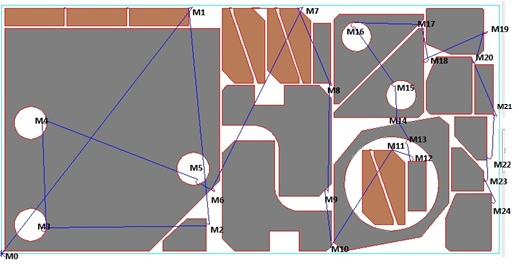
\includegraphics[width=0.9\textwidth]{cutting-24.png}
  \caption{
    Пример маршрута резки,
    содержащего 24 сегмента резки
  }
  \label{fig:cut.cutting}
\end{figure}

На рис. \ref{fig:cut.cutting}
показана схема одного из возможных маршрутов резки для примера,
приведенного на рис.~\ref{fig:cut.nesting}.
Маршрут содержит 24 сегмента.
Для резки внешних контуров трех групп деталей
с точками врезки $M_1$
(три детали в группе),
$M_7$
(четыре детали в группе) и
$M_{11}$
была использована мультиконтурная резка.
Все остальные контуры вырезаны с применением стандартной техники резки.
Последовательность резки сегментов соответствует
номерам точек врезки $M_j$ ($j=1,2,\,\dots, 24$).

Визуализация траектории инструмента
на рис.~\ref{fig:cut.cutting}
осуществляется точно по граничным контурам деталей,
а не по эквидистантным контурам,
в нарушение условия, что
траектория реза должна отстоять от
граничного контура.
Это связано с тем, что в большинстве
CAM-систем
программирование движения инструмента первоначально
осуществляется по граничным контурам деталей,
а вычисление реальной траектории производится
либо непосредственно самой системой ЧПУ,
либо специальной программой-постпроцессором,
предназначенной для конвертирования информации о
маршруте резки из внутреннего формата системы в
формат команд конкретного технологического оборудования с ЧПУ.

В дальнейшем мы будем полагать,
что траектория инструмента в маршруте резки $\mathfrak R$
программируется по граничным контурам,
и сегменты резки
$S_k=M_kM^*_k; k \in \overline{1,K}$
содержат все граничные контуры деталей
$C_1, C_2, \,\dots, C_N$,
т. е.
$$
\bigcup_{j=1}^N C_j \subset \bigcup_{k=1}^K S_k
$$

\begin{figure}
  \scriptsize
  \begin{multicols}{3}
    \%УП\_2Р32М\_01
    N1G91 \\
    N2G00X7662Y9909F6000 \\
    N3M70T1 \\
    N4M71T1 \\
    N5G01X-141Y-48F460 \\
    N6X-2400  \\
    N7X-40  \\
    N8X-67  \\
    N9X-2400  \\
    N10X-40 \\
    N11X-67 \\
    N12X-2400 \\
    N13Y-700  \\
    N14X2400  \\
    N15Y700 \\
    N16Y40  \\
    N17X107Y-40 \\
    N18Y-700  \\
    N19X2400  \\
    N20Y700 \\
    N21Y40  \\
    N22X107Y-40 \\
    N23Y-700  \\
    N24X2400  \\
    N25Y700 \\
    N26Y40  \\
    N27M74T1  \\
    N28G00X817Y-8745F6000 \\
    N29M71T1  \\
    N30G03X-108Y0I-54J0F460 \\
    N31G01Y-1048  \\
    N32X-1740 \\
    N33Y400 \\
    N34X940Y900 \\
    N35X800 \\
    N36Y-252  \\
    N37X20Y-30  \\
    \dots \\
    N314M71T1 \\
    N315G02X-130Y0I-65J0F460  \\
    N316G01Y267 \\
    N317G03X-50Y50I-50J0  \\
    N318G01X-1366 \\
    N319G03X-46Y-31I0J-50 \\
    N320G01X-384Y-960 \\
    N321G03X-4Y-19I46J-19 \\
    N322G01Y-1120 \\
    N323G03X14Y-35I50J0 \\
    N324G01X122Y-121  \\
    N325G03X37Y-14I35J35  \\
    N326G01X1627Y-1 \\
    N327G03X50Y50I0J50  \\
    N328G01Y1933  \\
    N329X20Y30  \\
    N330M74T1 \\
    N331M75T1 \\
    N332M02 \\
    M30
  \end{multicols}
  \caption{
    Фрагмент управляющей программы
    для машины листовой резки <<Комета>>~с~ЧПУ~2Р32М
  }
  \label{fig:cut.control-program}
\end{figure}

На рис.~\ref{fig:cut.control-program}
на стр.~\pageref{fig:cut.control-program}
показан фрагмент управляющей программы
(G-кода) для машины листовой газовой резки
типа <<Комета>> с системой ЧПУ~2Р32М.
Программа сгенерирована на основе маршрута резки
(спроектированного в интерактивном режиме в
CAD/CAM-системе <<Сириус>>
и показанного на рис.~\ref{fig:cut.cutting})
соответствующим постпроцессором со
следующими числовыми параметрами резки:
\begin{itemize}
  \item	число строк в УП – 333;
  \item	количество точек врезки – 24;
  \item	путь инструмента на рабочей скорости – 27,36 м;
  \item	путь инструмента на холостом ходу – 8,39 м;
  \item	время движения на рабочей скорости – 62,04 мин;
  \item	время движения на холостом ходу – 1,64 мин;
  \item	общее время резки: 63,68 мин.
\end{itemize}

В зависимости от выбранного маршрута резки
числовые параметры резки могут существенно различаться.
Таким образом, при разработке управляющих программ
для машин фигурной листовой резки с ЧПУ возникают
различные задачи оптимизации маршрута инструмента.
В качестве критерия оптимизации (целевой функции)
в этих задачах чаще всего рассматривается общее время резки
$T_{cut}$,
рассчитываемое по формуле:
\begin{equation}
  T_{cut} = \frac{L_{on}}{V_{on}} + \frac{L_{off}}{V_{off}} +N_{pt} \cdot t_{pt}
  ,
  \label{eq:cut.time}
\end{equation}
где
$L_{on}$ -- длина реза с включенным режущим инструментом;
$V_{on}$ -- скорость рабочего хода режущего инструмента;
$L_{off}$ -- длина переходов с выключенным режущим инструментом (холостой ход);
$V_{off}$ -- скорость холостого хода;
$N_{pt}$ -- количество точек врезки;
$t_{pt}$ -- время, затрачиваемое на одну точку врезки.

В~\eqref{eq:cut.time} значение скорости холостого хода инструмента
$L_{off}$ --- константа, определяемая техническими характеристиками
используемого технологического оборудования.
Значение скорости рабочего хода
$V_{on}$ программируется при разработке управляющей программы
в соответствии с используемой технологией резки и параметрами листового материала
(марка материала и толщина).
Предполагается, что заданная величина
$V_{on}$
в~\eqref{eq:cut.cost}
также является константой,
однако на практике фактическая скорость резки
может меняться в зависимости от различных технологических факторов,
а также характеристик спроектированной управляющей программы,
подробнее см.~\cite{bi:these.tavaeva}

Важнейшей экономической характеристикой качества
разработанной управляющей программы является стоимость
(себестоимость) резки деталей на машине с ЧПУ.
Это сложный интегрированный показатель,
который включает в себя произведенные во время
резки затраты на электроэнергию и расходные материалы,
на обслуживание машины с ЧПУ,
а также другие эксплуатационные затраты.
Стоимость резки не всегда
пропорциональна времени резки,
поскольку зависит еще и от различных режимов резки.
По аналогии с формулой времени резки \eqref{eq:cut.time}
показатель стоимости резки можно определить по следующей формуле:
\begin{equation}
  F_{cost}=
  L_{on} \cdot C_{on} +
  L_{off} \cdot C_{off} +
  N_{pt} \cdot C_{pt}
  ,
  \label{eq:cut.cost}
\end{equation}
где
$C_{on}$ -- стоимость единицы пути с включенным режущим инструментом;
$C_{off}$ -- стоимость единицы пути с выключенным режущим инструментом;
$C_{pt}$ -- стоимость одной точки врезки,
а $L_{on}, L_{off}, N_{pt}$
имеют тот же смысл, что и в формуле~\eqref{eq:cut.time}.
При этом величины $C_{on}, C_{off}, C_{pt}$
зависят от типа машины с ЧПУ,
технологии резки, используемой скорости рабочего хода инструмента,
толщины и марки материала.

Значения целевых функций \eqref{eq:cut.time}, \eqref{eq:cut.cost}
однозначно определяются маршрутом резки,
задаваемым кортежем \eqref{eq:cut.tuple},
поскольку геометрия сегментов резки
$S_1, S_2, \,\dots, S_K$
позволяет вычислить длину рабочего хода инструмента $L_{on}$,
а координаты точек
$M_0$, $M_1$, $M_1^*$, $M_2$, $M_2^*$, \,\dots, $M_K$, $M_K^*$
и перестановка
$i_1$, $i_2$, \,\dots, $i_K$
(последовательность, в которой вырезаются используемые сегменты резки)
задают набор холостых перемещений инструмента,
который определяет суммарную длину холостого хода
$L_{off}$.

Таким образом, сформулированные задачи оптимизации
маршрута инструмента для машин фигурной листовой резки с ЧПУ
можно представить в самом общем виде
как задачу минимизации некоторой числовой функции $\mathfrak F$
(например, \eqref{eq:cut.time} или \eqref{eq:cut.cost})
на множестве
$\mathfrak G$ допустимых кортежей
\eqref{eq:cut.tuple}:
\begin{equation}
  \mathfrak F(\mathfrak R) \to \min_{\mathfrak R \in \mathfrak G}
  \label{eq:cut.problem}
\end{equation}

Поскольку элементы кортежа содержат
(помимо последовательности резки
$i_1, i_2, \,\dots, i_K$,
выбираемой из дискретного множества перестановок)
точки врезки и точки выключения инструмента
$M_kM_k^*, k \in \overline{1,K}$,
которые, в свою очередь,
могут быть выбраны из континуальных подмножеств евклидовой плоскости
$\mathbb R \times \mathbb R$,
даже в случае наложения существенных ограничений
на возможность выбора допустимых сегментов
$S_k$
оптимизационная задача \eqref{eq:cut.problem}
может быть отнесена к классу очень сложных задач
непрерывно-дискретной оптимизации.
